\section{Teil \uproman{1}: Zeeman-Effekt}


\subsection{Aufbau}
    \begin{itemize}
        \item Justierung des Fabry-Perot-Etalon
        \item Aufbau der optischen Bank
        \item Strahlungsquelle \& Eigenschaften
    \end{itemize}
    
    \begin{figure}[H]
        \centering
        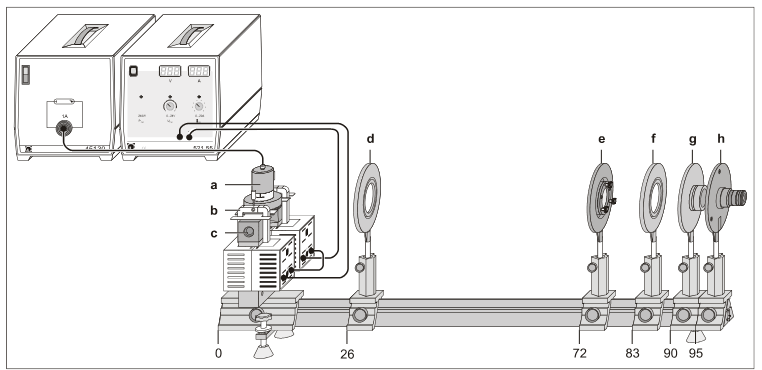
\includegraphics[width=0.65\linewidth]{figs/Zeeman_Aufbau.png}
        \caption{Aufbau in transversaler Konfiguration. \cite{Zeemann-Effekt_LD-Handblätter}}
    \end{figure}




\subsection{Beobachtung der Aufspaltung}
    \begin{itemize}
        \item Beobachtung $B = 0$ (1 Ring)
        \item Beobachtung $B \gg 0$ (3 Ringe)
        \item Beobachtung $B \gg 0$ mit Filter (1 oder 2 Ringe)
        \item Erklärung des Gesehenen
    \end{itemize}


    \begin{figure}[H]
        \centering
        \begin{subfigure}[t]{0.44\textwidth}
            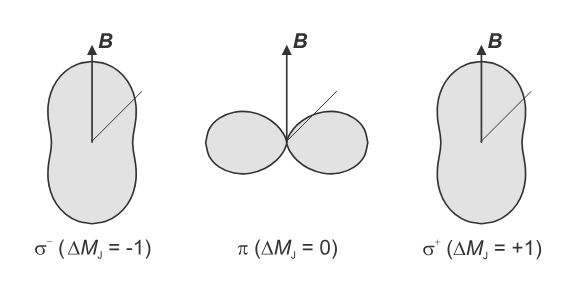
\includegraphics[width=\linewidth]{figs/Zeeman_B-Feld.png}
            \caption{}
        \end{subfigure}
        \hspace{0.2cm}
        \begin{subfigure}[t]{0.44\textwidth}
            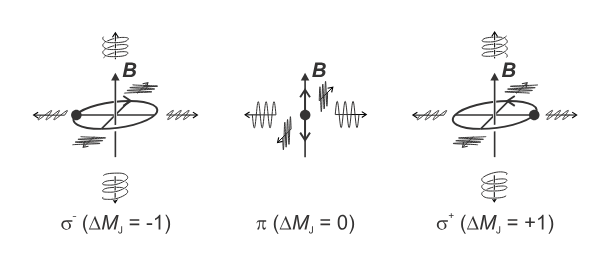
\includegraphics[width=\linewidth]{figs/Zeeman_Dipolstrahlung.png}
            \caption{}
        \end{subfigure}
        \caption{Winkelverteilung der elektrischen Dipolstrahlung. \cite{Zeemann-Effekt_LD-Handblätter}}
    \end{figure}



\subsection{Magnetfeld-Kalibrierung}
    \begin{itemize}
        \item Aufbau der Magnetfeld-Messung
        \item Ermittlung des Zusammenhang $B(I)$
        \item Ermittlung der Zusammenhangs $B(x)$
        \item vergleiche zweite Magnetfeld-Messung
        \item Diskussion Thermischer Effekte
    \end{itemize}

\subsection{Messung in Transversaler Konfiguration}
    \begin{itemize}
        \item Aufbau der Kamera und Aufnahme
        \item Spezifikationen der Kamera
        \item Beobachtung $B = 0$ (1 Ring)
        \item Beobachtung $B \gg 0$ (3 Ringe)
        \item Beobachtung $B \gg 0$ mit Filter (1 oder 2 Ringe)
        \item Erklärung des Gesehenen
    \end{itemize}




\subsection{Messung in Longitudinaler Konfiguration}
    \begin{itemize}
        \item Aufbau der Messung 
        \item Beobachtung $B = 0$ (1 Ring)
        \item Beobachtung $B \gg 0$ (2 Ringe)
        \item Beobachtung $B \gg 0$ mit Filter \& Platte (1 bis 2 Ringe)
        \item Erklärung des Gesehenen
    \end{itemize}
    
    
\subsection{Ergebnisse}
    \begin{itemize}
        \item Theoret. Abschätzung von Auflösung $\mathcal{A}$ und Finesse $\mathcal{F}$
        \item Experim. Bestimmung von Auflösung $\mathcal{A}$ und Finesse $\mathcal{F}$
        \item Umrechnung Pixel --> Winkel --> Wellenlänge
        \item Positionen \& Breiten der Maxima bestimmen
        \item Berechnung Energieverschiebung $\Delta E$
        \item Bestimmung Bohrschen Magnetons $\mu_B$
        \item Abschätzung von Doppler- und natürlicher Linienverbreiterung 
        \item Literaturvergleich
        \item Allgemeine Fehlerdiskussion 
    \end{itemize}


    \begin{figure}[H]
        \centering
        \begin{minipage}{0.35\textwidth}
            \centering
            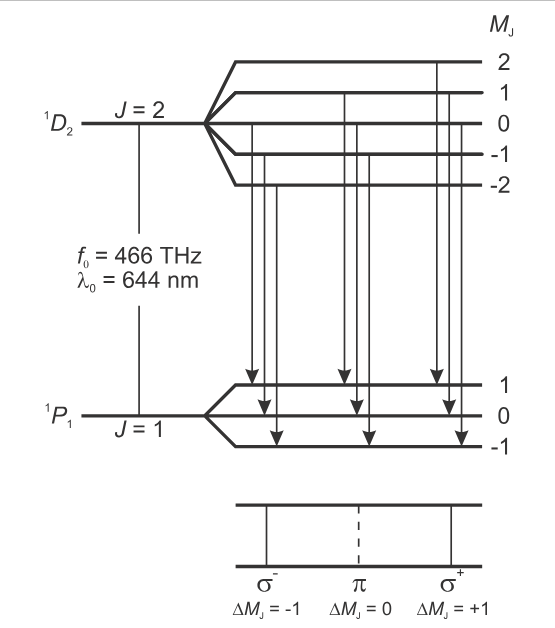
\includegraphics[width=\linewidth]{figs/Zeeman_Übergänge.png}
            \caption{Niveaufspaltung von Cadmium durch normalen Zeeman-Effekt. \cite{Zeemann-Effekt_LD-Handblätter}}
        \end{minipage} 
        \hspace{1cm}
        \begin{minipage}{0.4\textwidth}
            Text neben Abbildung...
        \end{minipage}
    \end{figure}


